\section{Incomplete Early-State Adaptation and Answer-Format Sensitivity}
\label{app:early-state-detail}
A separate adaptation shortened preparation to a 1,024-token source cap. Seven reader arms retained the complete graph and shared the same total-token allowance. The comparison included direct, question-first, Re2, task cue, prefix, append and a paid neutral prefix.

The runner ended without a terminal completion record. Later inspection confirmed its absence, but not the cause or exact termination time. The archive contained 149 qualified responses, including calibration and source calls, and one request-only record. Of 224 planned reader outputs, 129 were known. Known research usage was at least 3,621,241 tokens.

All-plan prefix F1 was bounded by $[0.34375,0.78125]$, compared with direct bounds $[0.19585,0.63335]$ (Figure~\ref{fig:early-state-interrupted}). These ranges represented missing outcomes, not sampling uncertainty. Seven of eighteen known prefix outputs were not normal-valid. Consequently, its required 31/32 normal-valid screening threshold was unattainable even if all remaining prefix outputs were valid.

\paragraph{Visible-answer sensitivity.} Five prefix failures reached the output limit; two normally stopped with surrounding prose. Direct reading had two output-limit failures and nine normally stopped malformed outputs. We separately accepted one unambiguous visible \texttt{Final Answer: [...]} line within surrounding prose, while still rejecting length termination and thinking-derived answers. This parser was post hoc and left primary scores unchanged.

On eighteen matched graph--seed outputs, prefix, direct and question-first each yielded thirteen exact answers under this sensitivity analysis. Re2 yielded fifteen, while task cue and neutral prefix yielded ten, and append yielded eleven. These incomplete counts did not establish equivalence or Re2 superiority. They showed that the apparent strict exact-match advantage over direct and question-first reading depended on the answer-format rule.

\begin{figure}[htbp]
\centering
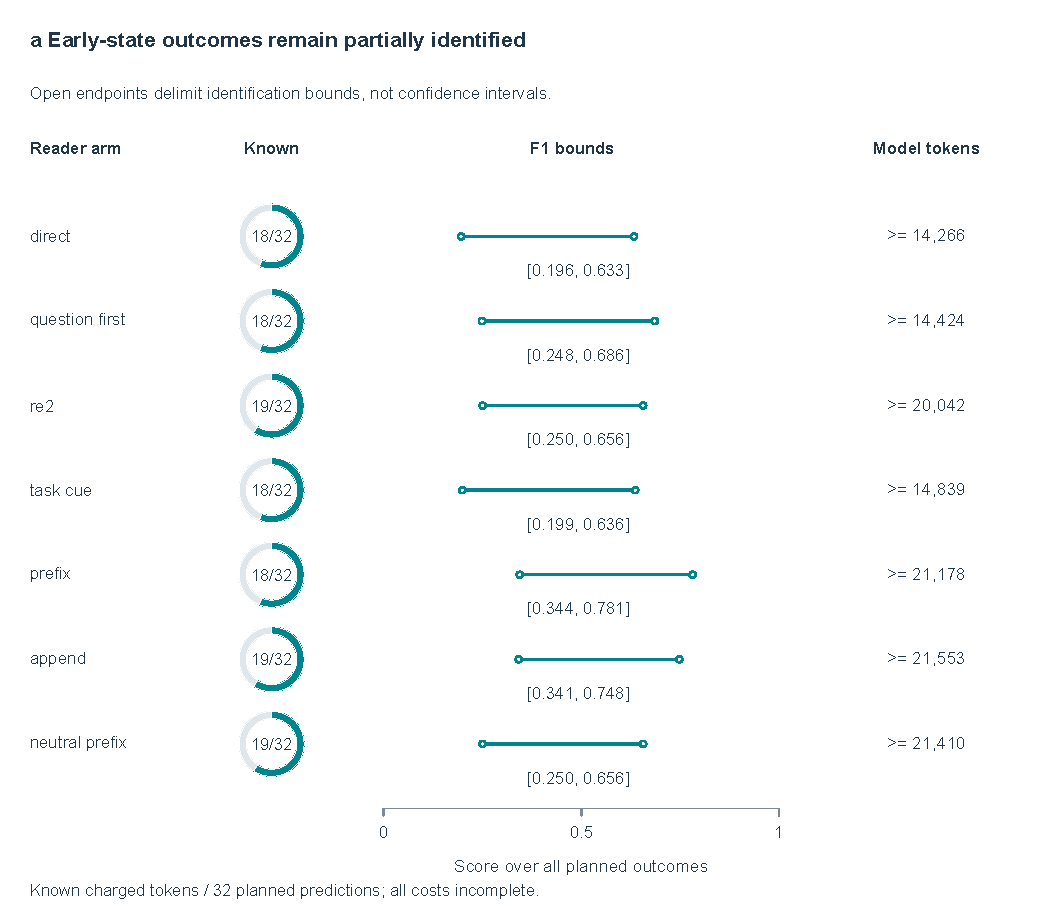
\includegraphics[width=\linewidth]{figures/refined_r_20261015/partial_state_display/publication.pdf}
\caption{Early-state adaptation after interrupted execution. Annular angles show known versus unknown outcomes for each arm, with all 32 planned outputs retained in the denominator. Open endpoints delimit F1 identification bounds and printed pairs give both endpoints; these are not sampling intervals. Cost labels marked $\geq$ give known charged deployment tokens divided by 32 planned predictions; every total is incomplete. Each state prediction pays full source cost. Unknown outcomes are not assigned failure scores. The ranges do not establish a quality gain or efficiency advantage.}
\label{fig:early-state-interrupted}
\end{figure}

